%%%%%%%%%% *** The Title %%%%%%%%%%
\title[]{수증기와 대기 안정도 \\ \small{제4장}}

\begin{frame}[plain] %title page
	\titlepage
\end{frame}


\begin{frame}[plain] %cc page
	\ccpage
\end{frame}


\section{지구상의 물}


\begin{frame}[t]{물순환(hydrologic cycle)}
	\begin{tabular}{ll}
		\begin{minipage}[t]{0.550\textwidth}
			\begin{figure}[t]
				\includegraphics[trim=40 10 285 475, clip, page=121, width=\textwidth]
				{\bookfile}
			\end{figure}
		\end{minipage}	
		&
		\begin{minipage}[t]{0.4\textwidth} \scriptsize
			\begin{itemize}
				\item 바다, 대기, 대륙 사이의 연속적인 물 교환
				\item 침투(infiltration) : 육지에 내린 비가 땅 속으로 스며드는 것
				\item 유출(runoff) : 육지에 내린 비가 지표면을 따라 흐르는 것
				\item 증발산(evapotranspiration) : 수면과 토양에서 증발과 식물의 증산을 합친 것
			\end{itemize}

		\end{minipage}
	\end{tabular}
\end{frame}




\begin{frame}[t]{물순환(hydrologic cycle)}
	\begin{tabular}{ll}
		\begin{minipage}[t]{0.40\textwidth}
			\begin{figure}[t]
				\includegraphics[trim=40 10 285 475, clip, page=121, width=\textwidth]
				{\bookfile}
			\end{figure}
		\end{minipage}	
		&
		\begin{minipage}[t]{0.55\textwidth} \scriptsize
			\questionset{주어진 그림을 참고하여 물순환 과정을 설명하시오.}
			\solutionset{바다 및 대륙에서 물의 증발로 대기권으로 수증기 유입되어, 강수가 형성될 때까지 수증기가 이동한다. \\
				바다로 내린 강수는 순환 종료되고, 육지로 내린 강수는 침투, 호수나 하천 유입 및 유출하게 되고, 지하수와 유출 대부분은 증발산 통해 대기권으로 다시 유입된다. \newline}
			
			\questionset{해양에서는 증발에 의해 감소되는 물의 양이 강수량과 같지 않다. 그런데도 해수면이 낮아지지 않는 이유는 무엇인가?}
			\solutionset{해양에서는 증발이 강수보다 많다. 차이가 나는 양은 대기를 통해 대륙으로 이동하여 강수의 형태로 내리게 된다. \\
			육지의 증발은 강수보다 적고 차이가 나는 물은 다시 바다로 흘러 들어가 전체 해수의 양은 보전된다. \newline}
		
			\questionset{물 순환의 의의에 대해 설명하시오.}
			\solutionset{잠열의 흡수와 방출을 통해 에너지를 수송한다.}
		\end{minipage}
	\end{tabular}
\end{frame}



\begin{frame}[t]{물의 특성}
	\begin{tabular}{ll}
		\begin{minipage}[t]{0.40\textwidth}
			\begin{figure}[t]
				\includegraphics[trim=40 400 290 50, clip, page=122, width=\textwidth]
				{\bookfile}
			\end{figure}
		\end{minipage}	
		&
		\begin{minipage}[t]{0.55\textwidth} \scriptsize
			\begin{itemize}
				\item 지구 표면에서 대량으로 발견되는 유일한 액체
				\item 한 상에서 다른 상(고체, 액체, 기체)으로 변환 가능함
				\item 고체 상태인 얼음은 액체 상태인 물보다 밀도가 작음
				\item 비열이 커서 온도 변화를 위해 많은 에너지가 요구됨
				\item 대다수의 특성은 물이 수소결합을 하는 특성의 결과임
			\end{itemize}
			
			\questionset{얼음이 물보다 밀도가 작은 이유를 설명하시오.}
			\solutionset{얼음은 가열되면 수소 결합의 일부가 끊어지며 녹는다. 그 결과 액체 속 물분자들은 좀 더 압축된(빽빽한) 배열을 가진다. 그러므로 액체 상의 물이 얼음보다 밀도가 더 크다.}
			
		\end{minipage}
	\end{tabular}
\end{frame}





\section{물의 상태변화}




\begin{frame}[t]{잠열}
	\begin{tabular}{ll}
		\begin{minipage}[t]{0.65\textwidth}
			\begin{figure}[t]
				\includegraphics[trim=40 400 70 50, clip, page=123, width=\textwidth]
				{\bookfile}
			\end{figure}
		\end{minipage}	
		&
		\begin{minipage}[t]{0.3\textwidth} \scriptsize
			\begin{itemize}
				\item 융해 잠열: $0 \rm{{^\circ}C}$의 얼음(고체)이 물(액체)로 변할 때 약 
				$80 \rm{~cal/g}$의 열을 흡수
				\item 기화 잠열: 물이 수증기로 변할 때는 $540 \rm{~cal/g} ~\left(100 \rm{{^\circ}C}\right) \sim600 \rm{~cal/g}~\left(0 \rm{{^\circ}C}\right)$의 열을 흡수함.
				\item 반대의 과정은 동일한 양의 열을 방출하는 것이 필요!
			\end{itemize}
			
		\end{minipage}
	\end{tabular}
\end{frame}





\begin{frame}[t]{상태 변화}
	\begin{tabular}{ll}
		\begin{minipage}[t]{0.60\textwidth}
			\begin{figure}[t]
				\includegraphics[trim=40 450 80 50, clip, page=124, width=\textwidth]
				{\bookfile}
			\end{figure}
		\end{minipage}	
		&
		\begin{minipage}[t]{0.35\textwidth} \scriptsize
			\begin{itemize}
				\item 증발: 액체 $\rightarrow$ 기체, 응결: 기체 $\rightarrow$ 액체
				\item 수증기가 구름을 형성할 때, 응결 잠열이 방출되며, 그 열이 주위 공기를 가열하여 공기 덩이에 부력을 주어 구름 성장에 도움을 줌
				\item 승화: 고체 $\rightarrow$ 기체, 침적: 기체 $\rightarrow$ 고체
				\item 승화에는 드라이아이스가 사라지는 현상이 대표적인 예이며, 침적은 수증기가 잔디나 창문 등에 얼음으로 침적되는 것(서리)이 예시임.
			\end{itemize}

		\end{minipage}
	\end{tabular}
\end{frame}





\section{습도: 공기 중의 수증기}





\begin{frame}[t]{공기 중의 수증기}
	\begin{tabular}{ll}
		\begin{minipage}[t]{0.50\textwidth}
			\begin{figure}[t]
				\includegraphics[trim=40 510 350 50, clip, page=125, width=\textwidth]
				{\bookfile}
			\end{figure}
		\end{minipage}	
		&
		\begin{minipage}[t]{0.45\textwidth} \scriptsize
			\begin{itemize}
				\item 기상학자들은 대기 중의 수증기량을 표현하기 위해 여러 방법들을 사용
			\end{itemize}
			\questionset{달톤의 법칙을 설명하시오.}
			\solutionset{기체들의 혼합물에 의한 전체 압력은 각 성분에 의한 분압의 합과 동일하다. \\
				$${\displaystyle	{ 
				p = p_{1}+p_{2}+\cdots + p_{k}=\sum_{1}^{k} p_{n}
				}	}$$ \newline}
		
			\questionset{수증기압이란 무엇인가?}
			\solutionset{전체 대기 압력에서 수증기가 기여한 압력을 수증기압(vapor pressure)라고 한다.}
		\end{minipage}
	\end{tabular}
\end{frame}




\begin{frame}[t]{수증기압과 포화}
	\begin{tabular}{ll}
		\begin{minipage}[t]{.475\textwidth}
			\begin{figure}{}
				\includegraphics[trim=30 410 290 170, clip, page=126, width=0.95\textwidth]{\bookfile} 
			\end{figure}
			\begin{itemize}\scriptsize
				\item 수증기압 : 전체 대기압력에서 수증기가  기여한 압력
				\item 포화 : 증발 속도 = 응결 속도
				\item 포화 수증기압: 포화되었을 때 수증기에 의해 가해진 압력
			\end{itemize}
		\end{minipage}
		&
		\begin{minipage}[t]{.475\textwidth}	
			\begin{figure}{}
				\includegraphics[trim=30 60 290 395, clip, page=126, width=0.95\textwidth]{\bookfile} 
			\end{figure}
		\end{minipage}
	\end{tabular}
	
\end{frame}




\begin{frame}[t]{절대습도(absolute humidity)}
	\begin{tabular}{ll}
		\begin{minipage}[t]{0.475\textwidth} \scriptsize
			혼합공기 $1 \rm{~m^3}$에 들어있는 수증기의 양을 $\rm{g}$으로 나타낸 것 \\
			$$ {\displaystyle	{
				\text { 절대습도 }=\frac{\text { 수증기 질량 }(\mathrm{g})}{\text { 공기 부피 }\left(\mathrm{m}^{3}\right)} 
			}	}$$
				
			이상기체 상태방정식으로 밀도를 구하면 
			$$ {\displaystyle	{
				e = {\rho} R T, \quad \rho = \frac{e}{R T}
			}	} $$
			와 같다. 수증기의 밀도($\rho_v$)는 
			$$ {\displaystyle	{
					\rho_{v}=\frac{e}{R_v T}
				} 	} $$
			$$ {\displaystyle	{
				\begin{aligned}
				R = M {\bar {R}} &= 8.3144 \left(\rm J~mol^{-1}~K^{-1}\right)  \\
				&= 8.3144 \left(\rm Pa~m^3~mol^{-1}~K^{-1}\right)
				\end{aligned}
				}	}	$$
		\end{minipage}	
		&
		\begin{minipage}[t]{0.475\textwidth} \scriptsize
			특별기체상수(specific gas constant)는 보편기체상수(${\bar{R}}$)를 기체의 분자량$\left(M\right)$으로 나누어 구할 수있다. 
			$$ {\displaystyle	{
				R = \frac{\bar{R}}{M}
			}	}	$$
			수증기의 기체상수는
				$$ {\displaystyle	{
				{{R_w}}={\frac {R}{M_w}} = {\frac {8.3144}{18}} = 0.461 \left(\rm J~g^{-1}~K^{-1}\right)
				}	}$$

				$$ {\displaystyle	{
						A. H.= \rho_{w}=\frac{e}{R_w T} = 217 \frac{e}{T} \left(\mathrm{g}~\mathrm{m}^{-3}\right)
				} 		} 	$$
				단, 여기에서 $\mathrm{e}: \mathrm{hPa}$, $\mathrm{T}: \mathrm{K}$ 단위이다. 
		\end{minipage}
	\end{tabular}
\end{frame}





\begin{frame}[t]{혼합비와 비습}
	\begin{tabular}{ll}
		\begin{minipage}[t]{0.475\textwidth} \scriptsize
			혼합비(Mixing Ratio) : 건조 공기 $1 \rm{~kg}$에 들어 있는 수증기의 양을 $ \rm{~g}$으로 나타낸 것
			\\
			$$ {\displaystyle	{
					\text { 혼합비 }=\frac{\text { 수증기 질량 }(\mathrm{g})}{\text { 건조 공기 질량 }(\mathrm{kg})} 
			} 		} 	$$		

			$$ {\displaystyle	{
				M.R.=\frac{m_{w}}{m_{d}}=\frac{\rho_{w}}{\rho_{d}} = 622 \frac{e}{p-e}(\mathrm{g} / \mathrm{kg})
			} 		} 	$$		
			이상기체 상태방정식을 이용해 구해볼 수 있다.
			$$ {\displaystyle	{
					\begin{aligned}
						p&=\rho R T, \quad \rho=\frac{p}{R T} \\
						e&=\rho_w R_w T, \quad \rho_w=\frac{e}{R_w T} \\
						M.R.&=\frac{\rho_w}{\rho_d} = \frac{\frac{e}{R_w T}}{\frac{\left(p-e\right)}{R_d T}} = \frac{M_w}{M_d}\frac{e}{p-e}
					\end{aligned}
			}	} $$
			

		\end{minipage}	
		&
		\begin{minipage}[t]{0.475\textwidth} \scriptsize
			비습(Specific Humidity) : 수증기와 혼합되어 있는  $1 \rm{~kg}$에 들어 있는 수증기의 양을 $ \rm{~g}$으로 나타낸 것 	\\
			$$ {\displaystyle	{
				\begin{aligned}
					&\text { 비습 }=\frac{\text { 수증기 질량 }(\mathrm{g})}{\text { 습윤 공기 질량 }(\mathrm{kg})} \\
					&S.H. = \frac{m_{w}}{m_{d}+m_{w}}=\frac{\rho_{w}}{\rho_{d}+\rho_{w}} = 622 \frac{e}{p}(\mathrm{g} / \mathrm{kg}) 
				\end{aligned}
			}		} 		$$	
		\end{minipage}
	\end{tabular}\end{frame}






\begin{frame}[t]{공기 중의 수증기}
	\begin{tabular}{ll}
		\begin{minipage}[t]{0.45\textwidth}
			\begin{figure}[t]
				\includegraphics[trim=330 50 50 440, clip, page=125, width=\textwidth]
				{\bookfile}
			\end{figure}
		\end{minipage}	
		&
		\begin{minipage}[t]{0.5\textwidth} \scriptsize
			\questionset{절대습도와 혼합비는 어떤 공통점과 차이점을 가지는가? }
			\solutionset{특정 양의 공기에 포함된 수증기의 양으로 표현된다는 점은 같으나, 절대 습도는 수증기의 양이 변하지 않음에도 불구하고 공기덩이의 부피 변화(단열 변화)에 따라 값이 변화하게 되지만, 혼합비는 수증기의 양이 변하지 않으면 변화하지 않는다는 점이 다르다. \newline}
			
			\questionset{상대 습도와 이슬점은 절대 습도, 혼합비와 어떻게 다른가? 상대 습도와 이슬점을 사용하는 이유는 무엇인가?}
			\solutionset{절대습도와 혼합비가 공기 중의 실제 수증기의 양을 나타내는 개념인데, 상대습도는 공기가 포화에 얼마나 근접해있는가를 나타내는 지표이다.\\
			절대습도와 혼합비를 직접 측정하기 어렵기 때문에 기상학에서 공기의 수분함유량을 표현하기 위해 주로 상대습도와 이슬점을 사용한다.}
		\end{minipage}
	\end{tabular}
\end{frame}







\begin{frame}[t]{포화 혼합비 곡선}
	\begin{tabular}{ll}
		\begin{minipage}[t]{.475\textwidth}
			\begin{figure}{}
				\includegraphics[trim=390 440 10 60, clip, page=126, width=0.95\textwidth]{\bookfile} 
			\end{figure}
		\end{minipage}
		&
		\begin{minipage}[t]{.475\textwidth}	
			\questionset{공기를 포화 시키는데 필요한 수증기량과 온도의 일반적인 관계를 기술하라.}
			\solutionset{오른쪽 포화 혼합비 곡선과 아래 포화 혼합비 표를 보면 보통 온도가 10℃ 상승하게 되면 포화수증기량이 약 2배씩 커진다.}
		\end{minipage}
	\end{tabular}
	
\end{frame}


\begin{frame}[t]{포화 혼합비}
	\begin{tabular}{ll}
		\begin{minipage}[t]{.45\textwidth}
			\begin{figure}{}
				\includegraphics[trim=400 40 30 490, clip, page=126, width=0.95\textwidth]{\bookfile} 
			\end{figure}
		\end{minipage}
		&
		\begin{minipage}[t]{.5\textwidth}	
			\questionset{이슬점이 $24\rm{{^\circ}C}$인 공기덩이는 이슬점이 이슬점이 $4\rm{{^\circ}C}$인 공기덩이 보다 얼마나 많은 수증기를 포함하고 있는가?}
			\solutionset{온도가 이슬점이 $10\rm{{^\circ}C}$씩 높아지면 수증기량도 보통 $2$ 배씩 증가하므로 이슬점이 $24\rm{{^\circ}C}$인 공기덩이는 이슬점이 이슬점이 $4\rm{{^\circ}C}$인 공기덩이보다 약 $4$배 많은 수증기를 포함하고 있을 것이다.}
		\end{minipage}
	\end{tabular}
	
\end{frame}







\section{상대습도와 노점온도}





\begin{frame}[t]{상대습도와 이슬점}
	\begin{tabular}{ll}
		\begin{minipage}[t]{0.475\textwidth} \scriptsize
			\begin{itemize}
				\item 		상대습도(Relative Humidity) : 특정 온도에서 포화되기 위해 필요한 수증기량과 실제 수증기량의 비율을 나타낸 것\\
				$$ {\displaystyle	{
						\begin{aligned}
							\text { 상대 습도 } &= \frac{\text {현재 수증기압 }(\mathrm{hPa})}{\text {포화 수증기압 }(\mathrm{hPa})} \times 100\left(\%\right) \\
							\text { 상대 습도 } &= \frac{\text {혼합비}(\mathrm{g/kg})}{\text {포화 혼합비}(\mathrm{g/kg})} \times 100\left(\%\right) 
						\end{aligned}
				} 		}		$$
				\item 		이슬점 : 포화되기 위해 냉각되어야 할 온도를 나타낸 것
			\end{itemize}			
		\end{minipage}	
		&
		\begin{minipage}[t]{0.475\textwidth} \scriptsize
				\questionset{서리점은 무엇인지 설명하시오.}
				\solutionset{온도가 $0\rm{{^\circ}C}$ 이하에서 포화가 일어나는 경우 서리점이라고 한다. 온도가 서리점 이하로 내려갈 경우 수증기는 액체를 거치치 않고 바로 침적되어 서리를 만든다.}		
			
		\end{minipage}
	\end{tabular}
\end{frame}






\begin{frame}[t]{상대습도}
	\begin{tabular}{ll}
		\begin{minipage}[t]{.46\textwidth}
			\begin{figure}{}
				\includegraphics[trim=270 50 30 410, clip, page=128, width=0.95\textwidth]{\bookfile} 
			\end{figure}
		\end{minipage}
		&
		\begin{minipage}[t]{.46\textwidth}	
			\begin{figure}{}
				\includegraphics[trim=50 375 230 50, clip, page=130, width=0.95\textwidth]{\bookfile} 
			\end{figure}
		\end{minipage}
	\end{tabular}
			\questionset{상대습도를 변화시키는 요인은 무엇인지 설명하시오}
			\solutionset{1) 수증기의 유입이나 제거, 2) 온도변화}
\end{frame}






\begin{frame}[t]{상대습도}
	\begin{tabular}{ll}
		\begin{minipage}[t]{.36\textwidth}
			\begin{figure}{}
				\includegraphics[trim=50 400 380 50, clip, page=131, width=0.95\textwidth]{\bookfile} 
			\end{figure}
		\end{minipage}
		&
		\begin{minipage}[t]{.59\textwidth}	
			\questionset{하루 중 상대습도가 가장 높았을 때와 가장 낮을 때는 언제인가}
			\solutionset{수증기량의 변화가 없다면 상대습도는 온도가 낮아 포화수증기량이 가장 낮은 새벽에 가장 높고, 온도가 가장 높은 오후에 가장 낮다. \newline}
			
			\questionset{하루 중 이슬이 생기기 쉬운 시간은?}
			\solutionset{이슬은 상대습도가 가장 높은 새벽에 나타나기 쉽다. \newline}
			
			\questionset{기온의 변화와 상대습도의 변화와의 일반적인 관계를 기술하라.}
			\solutionset{기온의 변화와 상대습도의 변화는 반비례한다. 즉 기온이 상승하면 상대습도는 하강하고, 기온이 하강하면 상대습도는 상승한다. \newline}
			
			\questionset{온도가 일정하고 혼합비가 감소한다면 상대습도는 어떻게 변하는가?}
			\solutionset{혼합비는 건조공기 $1 \rm{~kg}$에 들어있는 수증기의 양을 g으로 나타낸 것이고, 상대습도는 수증기량을 포화수증기량으로 나눈 것이다. \\
			그런데 혼합비가 감소하므로 수증기량은 감소하고, 온도는 일정하므로 포화 수증기량은 일정하기 때문에 상대습도는 감소한다.	}
		\end{minipage}
	\end{tabular}
\end{frame}





\begin{frame}[t]{상대습도와 수증기}
	\begin{tabular}{ll}
		\begin{minipage}[t]{.4\textwidth}
			\begin{figure}{}
				\includegraphics[trim=230 220 55 90, clip, page=129, width=0.95\textwidth]{\bookfile} 
			\end{figure}
		\end{minipage}
		&
		\begin{minipage}[t]{.55\textwidth}	
			\questionset{데스 밸리는 기온이 $25 \rm{{^\circ}C}$, 상대 습도는 20\% 이고, 시카고는 기온이 $-10 \rm{{^\circ}C}$, 상대 습도는 100\% 일 때, 두 지역에 포함된 수증기의 양을 비교하시오.}
			\solutionset{$-10 \rm{{^\circ}C}$의 포화 혼합비는 $2 \rm{~g/kg}$, $25 \rm{{^\circ}C}$의 포화 혼합비는 $20 \rm{~g/kg}$ 이므로 상대습도가 20\% 인 이 날 데쓰 밸리의 혼합비는 $4 \rm{~g/kg}$로 시카고보다 약 $2$배의 수증기를 포함한다.}
		\end{minipage}
	\end{tabular}
\end{frame}








\begin{frame}[t]{상대습도와 수증기}
	\begin{tabular}{ll}
		\begin{minipage}[t]{.4\textwidth}
			\begin{figure}{}
				\includegraphics[trim=50 50 250 420, clip, page=132, width=0.95\textwidth]{\bookfile} 
			\end{figure}
		\end{minipage}
		&
		\begin{minipage}[t]{.55\textwidth}	
			\questionset{건습계의 원리를 설명하라.}
			\solutionset{건습계는 일반적인 온도계인 건구 온도계와 구부가 물에 젖은 헝겊에 감싸여 있어 온도계를 돌리면서 증발이 일어나면서 에너지를 흡수하여 온도가 낮아지는 습구 온도계로 구성되어 있다. \\
			상대습도가 낮을수록 건구와 습구 온도의 차이가 커지게 되어 상대습도를 알 수 있다. \newline}
		
			\questionset{모발 습도계의 원리는 무엇이며, 단점과 장점은 무엇인가?}
			\solutionset{모발 습도계는 습도가 증가함에 따라 모발이 늘어나는 정도도 비례하여 증가한다는 원리를 이용한 습도계이다. \\
			단점은 건습계에 비해 정확하지 않고, 보정이 자주 필요하고, 특히 온도가 낮은 경우 습도 변화에 반응이 느리다는 점이고, 장점은 건습계는 건구 온도와 습구 온도를 모두 읽은 뒤 표에서 상대습도를 찾아야 하는 반면, 모발 습도계는 상대습도를 눈금으로 바로 읽으면 된다.}		
		\end{minipage}
	\end{tabular}
\end{frame}





\section{단열변화와 구름 형성}


\begin{frame}[t]{단열 변화}
	\begin{tabular}{ll}
		\begin{minipage}[t]{.4\textwidth}
			\begin{figure}{}
				\includegraphics[trim=35 440 290 50, clip, page=135, width=0.95\textwidth]{\bookfile} 
			\end{figure}
		\end{minipage}
		&
		\begin{minipage}[t]{.55\textwidth}	
			\questionset{공기가 대기를 통과하여 위쪽으로 상승하는 동안 공기는 왜 팽창하는지 설명하시오.}
			\solutionset{풍선과 같은 얇은 막을 가진 공기 덩이를 가정하자. 공기가 위로 상승하게 되면 기압이 감소하게 된다. 열의 출입이 없는 상태에서 공기덩이가 위로 상승하게 되면 공기덩이의 압력이 주위 공기의 압력보다 높게 되고, 부피가 증가하면서 일을 해주게 되면서 내부 에너지는 감소하고 기온도 감소하게 된다. \newline}
			
			\questionset{공기가 하강할 때는 왜 가열이 되는지 설명하시오.}
			\solutionset{공기가 하강하면 주변 공기의 압력이 공기덩이의 압력보다 크게 되어 공기덩이는 일을 받게 되고, 단열 상태에서 일을 받게 되면 내부에너지는 증가하여 기온은 상승하게 된다. \newline}
			
			\questionset{휴대용 부탄가스를 사용할때 용기가 차갑게 느껴지는 이유는?}
			\solutionset{내용물이 바깥으로 나오면서 압력이 낮아지고 일을 해주게 되어 내부에너지가 감소하게 되므로 기온이 내려가기 때문이다. \newline}					
		\end{minipage}
	\end{tabular}
\end{frame}



\begin{frame}[t]{단열 변화}
	\begin{tabular}{ll}
		\begin{minipage}[t]{.4\textwidth}
			\begin{figure}{}
				\includegraphics[trim=35 440 290 50, clip, page=135, width=0.95\textwidth]{\bookfile} 
			\end{figure}
		\end{minipage}
		&
		\begin{minipage}[t]{.55\textwidth}	
			\begin{itemize} \scriptsize 
				\item 	단열 변화 : 열의 출입이 없는 상태에서 일어나는 온도변화
				\item 	건조단열감률 : 연직으로 이동하는 불포화된 공기덩어리에 적용하는 온도감률 $10 \rm{{^\circ}C/km}$
				\item 	습윤단열감률 : 연직으로 이동하는 포화된 공기덩어리에 적용하는 온도감률 보통 수분함유량에 따라 약 $5\sim9 \rm{{^\circ}C/km}$
				\item 	이슬점감률 : 공기덩어리가 연직으로 이동하여 단열팽창하면 수증기의 밀도가 감소하여 수증기압도 낮아져서 이슬점이 내려감. 불포화 공기에서는 $2 \rm{{^\circ}C/km}$이며, 포화 공기에서는 해당 습윤단열감률과 동일함. 
			\end{itemize}	

		\end{minipage}
	\end{tabular}
\end{frame}



\begin{frame}[t]{상승 응결 고도}
	\begin{tabular}{ll}
		\begin{minipage}[t]{.4\textwidth}
			\begin{figure}{}
				\includegraphics[trim=335 40 30 350, clip, page=135, width=0.95\textwidth]{\bookfile} 
			\end{figure}
		\end{minipage}
		&
		\begin{minipage}[t]{.55\textwidth}
			\begin{itemize} \scriptsize 
				\item 불포화 상태인 공기가 상승 하여 포화에 도달해 구름이 형성되기 시작하는 고도
				\item 상승응결 고도를 $H$, 지상기온을 $t$, 지상 이슬점을 $t_d$라고 하면 건조 단열 감률은 $1 \rm{{^\circ}C/100~m}$, 이슬점 감률은 $0.2 \rm{{^\circ}C/100~m}$이므로, 
				$${\displaystyle {
					\begin{aligned}
					t-\left(H \times \frac{1^{\circ} \mathrm{C}}{100 \mathrm{m}}\right)&=t_{d}-\left(H \times \frac{0.2^{\circ} \mathrm{C}}{100 \mathrm{m}}\right) \\
					H[{m}]&=125\left({t}-{t}_{d}\right)
					\end{aligned}
				}	}$$
			\end{itemize}			
		\end{minipage}
	\end{tabular}
\end{frame}




\section{공기 덩이를 상승시키는 과정}


\begin{frame}[t]{지형성 상승}
	\begin{tabular}{ll}
		\begin{minipage}[t]{.5\textwidth}
			\begin{figure}{}
				\includegraphics[trim=50 40 220 450, clip, page=136, width=0.95\textwidth]{\bookfile} 
			\end{figure}
		\end{minipage}
		&
		\begin{minipage}[t]{.45\textwidth}
			\begin{itemize} \scriptsize 
				\item 공기덩이가 산악 장애물에 의해 강제 상승
				\item 푄 현상(높새 바람)
				\item 풍상측 경사면은 강수 유발
				\item 풍하측은 비그늘 사막(rain shadow desert)
			\end{itemize}	
			\questionset{겨울철에 강릉 지역이 왜 건조한지 설명하라.}
			\solutionset{겨울철 우리나라는 북서 계절풍이 주로 부는데 북서 계절풍이 산맥을 넘어오면서 수증기가 응결하여 많은 양의 수증기를 잃게 되어 혼합비가 낮아지고, 산맥을 넘어 풍하측인 강릉에 도착할때 단열압축을 하면서 더욱 따뜻한 공기덩이로 변하면서 상대습도가 낮아지게 된다.}
		\end{minipage}
	\end{tabular}
\end{frame}


\begin{frame}[t]{전선 치올림}
	\begin{tabular}{ll}
		\begin{minipage}[t]{.5\textwidth}
			\begin{figure}{}
				\includegraphics[trim=50 40 280 560, clip, page=137, width=0.95\textwidth]{\bookfile} 
			\end{figure}
		\end{minipage}
		&
		\begin{minipage}[t]{.45\textwidth}
			\begin{itemize} \scriptsize 
				\item 			따뜻하고 밀도가 작은 공기덩이가 차고 밀도가 큰 공기덩이 위로 강제 상승
			\end{itemize}	
			\questionset{전선 치올림이 공기를 상승시키는 과정을 설명하시오.}
			\solutionset{따뜻한 공기와 차가운 공기가 만나면 전선면을 만드는데, 밀도가 상대적으로 낮은 따뜻한 공기가 차가운 공기 위로 강제로 올라가면서 단열변화가 나타나게 된다.}

		\end{minipage}
	\end{tabular}
\end{frame}




\begin{frame}[t]{수렴}
	\begin{tabular}{ll}
		\begin{minipage}[t]{.45\textwidth}
			\begin{figure}{}
				\includegraphics[trim=50 440 300 50, clip, page=138, width=0.85\textwidth]{\bookfile} 
			\end{figure}
		\end{minipage}
		&
		\begin{minipage}[t]{.5\textwidth}	
			\begin{figure}{}
				\includegraphics[trim=350 440 50 50, clip, page=138, width=0.75\textwidth]{\bookfile} 
			\end{figure}
		\end{minipage}
	\end{tabular}
		\begin{itemize} \scriptsize 
			\item 			수평적 공기 흐름에 의해 쌓인 공기가 상승
		\end{itemize}
	\questionset{수렴이 공기를 상승시키는 과정을 설명하시오.}
	\solutionset{지표면 근처의 바람이 일정 영역에서 빠져 나가는 것보다 더 많이 들어오게 되면, 이를 수렴이라 하며 이 때 상승이 발생한다. }

\end{frame}





\begin{frame}[t]{국지적 대류 치올림}
	\begin{tabular}{ll}
		\begin{minipage}[t]{.9\textwidth}
			\begin{figure}{}
				\includegraphics[trim=50 40 70 530, clip, page=138, width=0.95\textwidth]{\bookfile} 
			\end{figure}
		\end{minipage}
		&
		\begin{minipage}[t]{.05\textwidth}	
			
		\end{minipage}
	\end{tabular}

		\questionset{국지적 대류성 치올림은 공기를 상승시키는 원인이 되는 다른 세 과정과 다르다. 어떻게 다른지 설명하시오.}
		\solutionset{다른 세 과정이 강제적인 요인으로 인해 공기의 상승이 시작됨에 반하여 국지적 대류성 치올림은 공기덩이의 온도가 주변보다 높아서 자발적으로  일어나는 상승이라는 측면에서 다르다.}

\end{frame}






\section{날씨 조절 중요인자: 대기안정도}


\begin{frame}[t]{대기안정도}
	\begin{tabular}{ll}
		\begin{minipage}[t]{.4\textwidth}
			\begin{figure}{}
				\includegraphics[trim=350 40 50 450, clip, page=140, width=0.95\textwidth]{\bookfile} 
			\end{figure}
		\end{minipage}
		&
		\begin{minipage}[t]{.55\textwidth}	
			\questionset{대기안정도의 엄밀한 정의를 설명하시오.}
			\solutionset{정적 안정도를 의미하는 것으로, 평형상태(정지상태)에서 어떤 변화가 생겼을 때 변화가 계속하여 나타나면 불안정, 원래의 정지상태로 돌아가면 안정이라고 판단하는 것이다. 참고로 대기안정도는 일반적으로 대기의 수직운동에 초점을 맞춘다. \newline}
			
			\questionset{대기안정도를 결정하는 기준은 무엇인가?}
			\solutionset{대기안정도는 어떤 높이에서 특정 공기덩어리의 기온과 그 높이에서의 실제 대기 기온의 크기를 비교하여 결정하는 것이 아니고, 대기안정도는 환경기온감률이 건조단열감률, 습윤단열감률에 비해 어떤 크기를 갖느냐에 따라 결정된다.\newline}
			
			\questionset{환경기온감률(environmental lapse rate)과 단열감률의 차이점을 설명하라.}
			\solutionset{환경기온감률이란 지표로부터 멀어질수록 지표면에서 방출되는  지구복사가 감소하여 점차 기온이 낮아지는 경향에 따라 실제로 나타나는 고도에 따른 기온의 변화율을 말한다. \\
			반면 단열감률은 공기덩이가 연직방향으로 움직일 때 공기덩이가 경험하게 되는 온도 변화를 말한다.}
		
		\end{minipage}
	\end{tabular}
\end{frame}



\begin{frame}[t]{절대 안정}
	$\text{환경기온감률} < \text{습윤단열감률}$
	
	\begin{tabular}{ll}
		\begin{minipage}[t]{.7\textwidth}
			\begin{figure}{}
				\includegraphics[trim=50 410 70 60, clip, page=141, width=\textwidth]{\bookfile} 
			\end{figure}
		\end{minipage}
		&
		\begin{minipage}[t]{.25\textwidth}
			공기의 연직방향 이동이 잘 일어나지 않으므로 층운형(stratus)의 구름이 형성되고, 흐리거나 약한 비가 내린다. 
		\end{minipage}
	\end{tabular}

\end{frame}



\begin{frame}[t]{절대 불안정}
		$\text{환경기온감률} > \text{습윤단열감률}$
	\begin{tabular}{ll}
		\begin{minipage}[t]{.7\textwidth}
			\begin{figure}{}
				\includegraphics[trim=50 40 70 440, clip, page=141, width=\textwidth]{\bookfile} 
			\end{figure}
		\end{minipage}
		&
		\begin{minipage}[t]{.25\textwidth}	
			공기의 연직방향 이동이 활발하게 일어나므로 적운형(cumulus)의 구름이 형성되고, 소나기가 내린다.
			
		\end{minipage}
	\end{tabular}
\end{frame}


\begin{frame}[t]{조건부 불안정}
	$\text{습윤단열감률} < \text{환경기온감률} < \text{습윤단열감률}$
	\begin{tabular}{ll}
		\begin{minipage}[t]{.65\textwidth}
			\begin{figure}{}
				\includegraphics[trim=50 340 70 50, clip, page=142, width=\textwidth]{\bookfile} 
			\end{figure}
		\end{minipage}
		&
		\begin{minipage}[t]{.3\textwidth}	\scriptsize 
			공기의 강제적 상승이 일어나면 층운형 구름이 만들어 지다가 주변의 기온보다 높아지면 스스로 상승하여 적운형 구름이 만들어진다. 
			
			
		\end{minipage}
	\end{tabular}
\end{frame}


\begin{frame}[t]{대기 안정도}
	\begin{tabular}{ll}
		\begin{minipage}[t]{.9\textwidth}
			\begin{figure}{}
				\includegraphics[trim=50 290 50 50, clip, page=143, width=0.7\textwidth]{\bookfile} 
			\end{figure}
		\end{minipage}
		&
		\begin{minipage}[t]{.05\textwidth}	
			
		\end{minipage}
	\end{tabular}
\end{frame}




\begin{frame}[t]{안정도의 변화}
	\begin{tabular}{ll}
		\begin{minipage}[t]{.75\textwidth}
		\questionset{조건부 불안정에서 ‘조건부’가 의미하는 바는 무엇인가?}
		\solutionset{조건부 불안정 상태에 있는 공기덩이는 현재는 불포화 상태이며 환경기온감률이 (건조)단열감률보다는 작기 때문에 안정한 상태이다.\\
			하지만 강제적으로 상승을 시켜서 포화 상태가 되면 환경기온감률이 (습윤)단열감률보다는 크기 때문에 불안정한 상태가 된다. 즉, 특정 조건이 만족되어야만 불안정한 상태가 된다는 의미를 뜻한다. \newline}
		
		\questionset{불안정도를 강화시킬 수 있는 네 가지 방법을 제시하라.}
		\solutionset{기본적으로 지표 근처의 공기를 가열시키면 된다.\\
			1) 지표의 강한 가열\\
			2) 따뜻한 지표면을 가로지르는 것과 같은 지표로 인한 기단의 가열\\
			3) 공기덩이의 상승\\
			4) 구름 꼭대기에서의 복사 냉각 \newline}
		
		\questionset{안정도를 강화시킬 수 있는 세 가지 방법을 제시하라.}
		\solutionset{기본적으로 지표 근처의 공기를 냉각시키면 된다.\\
			1) 일몰 후 지표면의 복사 냉각\\
			2) 찬 지표면을 가로지르는 것과 같은 지표로 인한 기단의 냉각\\
			3) 공기덩이의 침강 }

		\end{minipage}
		&
		\begin{minipage}[t]{.2\textwidth}	
		\end{minipage}
	\end{tabular}
\end{frame}




\section{안정도와 날씨}




\begin{frame}[t]{대기 안정도}
	\begin{tabular}{ll}
		\begin{minipage}[t]{.55\textwidth}
			\begin{figure}{}
				\includegraphics[trim=210 30 50 520, clip, page=144, width=0.95\textwidth]{\bookfile} 
			\end{figure}
		\end{minipage}
		&
		\begin{minipage}[t]{.4\textwidth}	
			\questionset{적운의 상층부를 보고 대기 안정도를 판단하시오.}
			\solutionset{적운 상층부를 보면 위쪽으로 계속해서 상승하려는 모습을 보이는 것으로 보아 기층이 매우 불안정하여 상승하면서 응결하고 있으며, 적운 아래쪽에는 소나기가 내리는 모습을 확인할 수 있다. }
		\end{minipage}
	\end{tabular}
\end{frame}




\begin{frame}[t]{지형 효과}
	\begin{tabular}{ll}
		\begin{minipage}[t]{.55\textwidth}
			\begin{figure}{}
				\includegraphics[trim=285 470 55 90, clip, page=145, width=0.95\textwidth]{\bookfile} 
			\end{figure}
		\end{minipage}
		&
		\begin{minipage}[t]{.4\textwidth}	
			\questionset{지형성 상승이 공기의 온도를 상승시키는 과정을 설명하시오.}
			\solutionset{산맥과 같은 높은 지형이 공기 흐름을 막게 되고 공기는 산맥의 경사면을 따라 상승하게 되면서 기압 하강에 따라 단열변화가 나타나게 된다. 상승응결고도 이후 수증기가 응결하게 되면 잠열을 방출하여 습윤단열감율로 변화하고, 풍상측에는 비를 뿌리는 경우가 많다. \\
			산을 넘어 하강할때는 건조단열감률로 온도가 상승하여 풍하측에는 고온 건조한 바람이 불게 된다. }
		\end{minipage}
	\end{tabular}
\end{frame}




\begin{frame}[t]{지리적 위치}
	\begin{tabular}{ll}
		\begin{minipage}[t]{.55\textwidth}
			\begin{figure}{}
				\includegraphics[trim=90 300 70 50, clip, page=146, width=\textwidth]{\bookfile} 
			\end{figure}
		\end{minipage}
		&
		\begin{minipage}[t]{.4\textwidth}	
		\questionset{오른쪽 그림에서 바람은 주로 어느쪽으로 부는지 설명하시오.}
		\solutionset{산맥의 서쪽이 동쪽에 비해 강수량이 많은 것으로 보아 서풍이 부는 지역이라고 생각할 수 있다. \newline}
		
		\questionset{겨울철에 강릉 지역이 왜 건조한지 설명하시오.}
		\solutionset{겨출철 우리나라는 북서 계절풍이 불고, 강릉은 태백산맥의 풍하측에 존재하게 되는데 산맥을 넘어오면서 수증기가 응결하여 많은 양의 수증기를 잃게 되어 혼합비가 낮아진 채로 공기덩이가 산맥을 넘어 오게 되고, 단열압축을 하면서 더욱 따뜻하고 공기덩이로 변하면서 상대습도가 낮아지게 된다. }
		
	
		\end{minipage}
	\end{tabular}
\end{frame}


\begin{frame}[t]{기온 역전과 안정도}
	\begin{tabular}{ll}
		\begin{minipage}[t]{.4\textwidth}
			\begin{figure}{}
				\includegraphics[trim=350 350 50 50, clip, page=144, width=0.9\textwidth]{\bookfile} 
			\end{figure}
		\end{minipage}
		&
		\begin{minipage}[t]{.55\textwidth}	
			\questionset{사진과 같이 발전소의 굴뚝을 높게 설치하는 이유는 무엇인가?}
			\solutionset{접지 역전층의 경계보다 높게 설치해야 지표면에서의 대기오염 피해를 줄일 수 있다.}
			
		\end{minipage}
	\end{tabular}
\end{frame}





\begin{frame}[t]{접지 역전}
	\begin{tabular}{ll}
		\begin{minipage}[t]{.55\textwidth}
			\begin{figure}{}
				\includegraphics[trim=30 450 350 50, clip, page=147, width=0.95\textwidth]{\bookfile} 
			\end{figure}
		\end{minipage}
		&
		\begin{minipage}[t]{.4\textwidth}
			\begin{itemize} \scriptsize 
				\item 지표근처에서 발생하는 역전층
				\item 복사 역전: 야간동안 지표의 복사냉각으로 인해 지표면에 접한 공기가 상층보다 더 냉각되어 형성
				\item 이류역전: 따뜻한 공기가 찬 지표 혹은 수면,설면을 지날 때 기층이 밑에서 부터 냉각되어 형성
			\end{itemize}	
		\end{minipage}
	\end{tabular}
\end{frame}







\begin{frame}[t]{상층 역전}
	\begin{tabular}{ll}
		\begin{minipage}[t]{.5\textwidth}
			\begin{figure}{}
				\includegraphics[trim=30 50 350 350, clip, page=147, width=0.95\textwidth]{\bookfile} 
			\end{figure}
		\end{minipage}
		&
		\begin{minipage}[t]{.45\textwidth}	
			
			\begin{itemize} \scriptsize 
				\item 대기 상층에서 발생하는 역전층
				\item 침강 역전: 고기압 구역에서 기층 전체가 서서히 침강하면서 단열변화에 의해 역전층 형성
				\item 전선 역전: 따뜻한 공기가 찬 공기 위를 타고 상승하는 전선면 부근의 전이층(기온 변화가 급격히 일어나는 층)에서 발생
				\item 해풍 역전: 해풍을 이루는 비교적 찬 공기와 육지의 따뜻한 공기 사이에서 전선면이 뚜렷하게 발생하는데, 이 전선면의 전이층에서도 기온 역전이 발생
			\end{itemize}
			
	
		\end{minipage}
	\end{tabular}
\end{frame}




\section{추가 내용}



\begin{frame}[t]{이상기체 상태방정식}
	\begin{tabular}{l|l}
		\begin{minipage}[t]{0.475\textwidth} \scriptsize 
			온도 $T$와 압력 $p$ 에서 이상기체의 단위질량 당 부피인 비부피를 $\nu$라 하자.
				그러면 보일의 법칙, 샤를의 법칙, 보일-샤를의 법칙을 다음과 같이 나타낼 수 있다.
				$$	{\displaystyle	{
						p \nu(T,~p)=p_{0} \nu\left(T, p_{0}\right),
						\quad 
						\frac{\nu \left(T, p_{0}\right)}{T}=\frac{\nu \left(T_{0}, p_{0}\right)}{T_{0}}
				}	}$$
				$${\displaystyle	{
						p \nu(T, ~p)=\frac{p_{0} \nu \left(T_{0}, ~p_{0}\right)}{T_{0}} T
				}	}$$
				비기체상수(specific gas constant) $R$을 이용하여 다음과 같이 쓸 수 있다.\\
				$${\displaystyle	{
						p \nu = R T
				}	}$$
				질량이 분자량 $M$과 같은 기체의 시료가 있다면 부피는 $V = M\nu$ 이다.\\
				$${\displaystyle	{
						pV= MR T 
				}	}$$	
		\end{minipage}
		&
		\begin{minipage}[t]{0.475\textwidth} \scriptsize 
			경험 법칙인 아보가드로의 법칙은 동일한 압력과 온도에서 같은 부피 안에 같은 수의 분자수를 지니므로 $\bar R = MR$의 양은 모든 기체에서 상수가 되며 이를 보편기체상수라 한다.
			$$ M R = \frac{pV}{T}, \quad p\nu= \frac{\bar {R}}{M} T $$
			$$ \bar R = MR = 8.3144 \left(\rm J mol^{-1} K^{-1}\right) $$
			
			비기체상수(specific gas constant)는 보편기체상수를 기체의 분자량으로 나누어 구할 수있다. \\
			$$R = \frac{\bar{R}}{M}$$
			이상 기체 상태방정식은 아래와 같이 쓸 수도 있다.\\
			$$p  =  \rho R T$$
			
		\end{minipage}
	\end{tabular}
\end{frame}




\begin{frame}[t]{공기의 평균 분자량}
	\begin{tabular}{l|l}
		\begin{minipage}[t]{0.475\textwidth} \scriptsize 
			공기의 부피를 $V$, $n$ 번째 기체의 질량을 $m_n$ , 분자량을 $M_n$ 이라고 하자
				$$	{\displaystyle	{
						p_{n}=\frac{\bar{R}}{M_{n}} \frac{m_{n}}{V} T
				} 	}	$$
				달톤의 법칙을 적용하면 \\
				$$	{\displaystyle	{
					\begin{aligned}
						p&=\sum p_{n}=\frac{\bar{R} T}{V} \sum \frac{m_{n}}{M_{n}}\\
						p \nu &=\bar{R} T \frac{\sum \frac{m_{n}}{M_{n}}}{\sum m_{n}}\\
						p \nu&=\frac{\bar{R}}{\bar{M}} T
					\end{aligned}
				}	}	$$

				량은 다음과 같이 정의된다. \\
				$$	{\displaystyle	{
						\frac{1}{\bar{M}} \equiv \frac{\sum \frac{m_{n}}{M_{n}}}{\sum m_{n}}
				}	}	$$
			
		\end{minipage}
		&
		\begin{minipage}[t]{0.475\textwidth} \scriptsize 
			
			혼합 기체인 공기의 평균 분자량은 질량 가중값을 사용하는 조화 평균으로 구할 수 있다.\\

			계산된 건조 공기의 평균 분자량은 $28.966 \times 10^{-3} \rm{~kg~{mol}^{-1}}$ 이다. \\
			건조 공기의 비기체상수는
			$${\displaystyle	{
					R = \frac{\bar{R}}{\bar{M}}=2.8704 \times 10^{2} \rm{~J~{kg}^{-1}~{K}^{-1}}
			}	}$$
			
		\end{minipage}
	\end{tabular}
\end{frame}




\begin{frame}[t]{정적 비열과 정압 비열}
	\begin{tabular}{l|l}
		\begin{minipage}[t]{0.475\textwidth} \scriptsize
			비열은 어떤 물질 $1 \rm{g}$의 온도를 $1 \rm{{^\circ}C}$ 올리는데 필요한 열량이다. \\
			정적비열 ($C_v$): 부피를 일정하게 유지하면서 가열했을 때 물질이 나타내는 비열 \\
			정압비열 ($C_p$): 압력을 일정하게 유지하면서 가열했을 때 물질이 나타내는 비열 \\
			내부에너지 $U$는 사실상 온도와 부피의 함수이며 압력과는 무관하다. \\
			따라서 $U \left(T, V\right)$로 나타낸다. \\
			엔탈피는 온도와 압력에 관한 함수로 $H \left(T, P\right)$로 나타낼 수 있는데, 정의는 $H =  U + PV$ 이다.\\
			정적 비열과 정압 비열을 각각 내부에너지와 엔탈피를 이용하여 표현하면 다음과 같다. \\
			$${\displaystyle	{
					C_{v}=\left(\frac{\partial U}{\partial T}\right)_{v}
					\quad	C_{p}=\left(\frac{\partial H}{\partial T}\right)_{p}
			}	}$$
		\end{minipage}	
		&
		\begin{minipage}[t]{0.475\textwidth} \scriptsize
			$${\displaystyle		{
					\begin{aligned} 
						C_{p} &=\left(\frac{\partial H}{\partial T}\right)_{p} =\left(\frac{\partial(U+P V)}{\partial T}\right)_{p} \\ &=\left(\frac{\partial U}{\partial T}\right)_{p}+P\left(\frac{\partial V}{\partial T}\right)_{p} \\ 
						&=C_{v}+P\left(\frac{\partial\left(\frac{R T}{P}\right)}{\partial T}\right)_{p} =C_{v}+P\left(\frac{R}{P}\right) \\ 
						&=C_{v}+R 
					\end{aligned}
			}	}$$
			
			따라서 정압 비열과 정적 비열사이의 관계는 $C_{p} = C_{v} + R$로 정리할 수 있다.
		\end{minipage}
	\end{tabular}
\end{frame}




\begin{frame}[t]{열역학 제1법칙}
	\begin{tabular}{l|l}
		\begin{minipage}[t]{.475\textwidth} \scriptsize 
			열역학 제 1법칙을 이용하여 ${\Delta q=c_{v} \Delta T+p \Delta \nu}$을 설명하면\\
			어떤 공기덩이에 열량 $\Delta Q$를 가하면 이중 일부는 $\Delta W$ 만큼의 일을 하는데 사용되고, 나머지는 $\Delta U$ 만큼의 내부에너지를 변화시키는데 사용된다.\\
				$$\Delta Q=\Delta U+\Delta W$$
				각 항을 공기덩이의 질량으로 나누어 단위 질량에 대해 다음과 같이 소문자로 나타내면 \\
				$$\Delta q=\Delta u+\Delta w$$
				이상기체라고 가정하면 \\
				$$\Delta u=c_{v} \Delta T$$
				여기에서 $c_{v}$는 정적비열이고, $\Delta T$는 온도 변화량이다.
		\end{minipage}
		&
		\begin{minipage}[t]{.475\textwidth}	\scriptsize 
			일의 물리학적 정의는 
			$${\Delta W=F \Delta S}$$
			반지름 $R$ 인 공 모양의 공기덩이의 압력을 $p$, 그 표면적을 $A$라 하면 
			$${\Delta W = p A \Delta R = p \Delta V}$$
			단위 질량의 공기덩이인 비부피에 대해 다음과 같이 쓸 수 있다. 
			$${\Delta w = p \Delta \nu}$$
			이를 대입하면 ${\Delta q=c_{v} \Delta T+p \Delta \nu}$ 이다.
			
		\end{minipage}
	\end{tabular}
\end{frame}







\begin{frame}[t]{열역학 제1법칙}
	\begin{tabular}{l|l}
		\begin{minipage}[t]{0.475\textwidth} \scriptsize
			${\Delta q=c_{v} \Delta T+p \Delta \nu}$을 ${\Delta q = c_{p} \Delta T - \nu  \Delta p}$로 표현하자면 \\
			공기덩이의 압력이 $p \rightarrow p+\Delta p$, 비부피가 $\nu \rightarrow \nu +\Delta \nu $, 온도가 $T \rightarrow T +\Delta T$로 변화했다면 나중 상태의 상태방정식은 \\
				$${\displaystyle {
						(p+\Delta p)(\nu+\Delta \nu)=R (T+\Delta T)
				} }$$
				$${\displaystyle {
						\\
						p \nu\left(1+\frac{\Delta p}{p}+\frac{\Delta \nu}{\nu}+\frac{\Delta p \Delta \nu}{p \nu}\right)=R T\left(1+\frac{\Delta T}{T}\right)
				} }$$
				
				$p \nu =R T$를 사용하고, $\frac{\Delta p}{p}$, $\frac{\Delta \nu}{\nu}$가 $1$보다 훨씬 작은 양으로 취급하여 $\frac{\Delta p \Delta \nu}{p \nu}$	항을 무시하면\\
				$${\displaystyle {
						\frac{\Delta T}{T}=\frac{\Delta p}{p}+\frac{\Delta \nu}{\nu}
				}		}$$	
		\end{minipage}	
		&
		\begin{minipage}[t]{0.475\textwidth} \scriptsize
			우변에 $RT$를 곱하고, 좌변에 ${p \nu}$를 곱하면\\
			$${\displaystyle {
				\begin{aligned}
					R \Delta T&= \nu \Delta p+p \Delta \nu \\
					p \Delta \nu &= R \Delta T - \nu \Delta p \\
					\Delta q&=c_{v} \Delta T+p \Delta \nu \\
					&= (c_{v}+R) \Delta T - \nu \Delta p
				\end{aligned}
			} 	}$$
		$c_p = c_v+R$ 이므로	\\
		$${\Delta q = c_{p} \Delta T - \nu  \Delta p}$$
		\end{minipage}
	\end{tabular}
\end{frame}






\begin{frame}[t]{건조단열감률}
	\begin{tabular}{l|l}
		\begin{minipage}[t]{0.475\textwidth} \scriptsize
			열역학 제1법칙 $\Delta q = c_{p} \Delta T - \nu  \Delta p$을 미분형으로 쓰면 
				$$	{\displaystyle	{
					d q = c_{p} d T - \nu  d p
				}	}	$$
			단열 변화에서는 $d q = 0$이고, 대기의 정역학적 평형 $dp = - \rho g dz$을 고려하면
				$${\displaystyle	{
					\begin{aligned}
						0 &= c_{p} d T - \nu  d p \\
						0 &= c_{p} d T + g  d z
					\end{aligned}
				}	}	$$		
			식을 정리하면
				$${\displaystyle	{
					- \frac {dT}{dz} = \frac{g}{c_p} = {\Gamma}_{d}
				}	}$$	
		\end{minipage}	
		&
		\begin{minipage}[t]{0.475\textwidth} \scriptsize
			
			
		\end{minipage}
	\end{tabular}
\end{frame}



\begin{frame}[t]{습윤단열감률}
	\begin{tabular}{l|l}
		\begin{minipage}[t]{0.475\textwidth} \scriptsize
			포화 공기는 수증기 응결로 인해 잠열이 방출되므로  $d q \neq 0$ 이다.\\
			포화혼합비를 $W_s$라고 하고, 응결 숨은열을 $L$이라고 하면 
			응결에 의해 단위 질량의 건조 공기가 흡수하는 열량은 $-Ldw_s$이다.
				$${\displaystyle	{
					-Ldw_s = c_{p} d T + gdz
				}	}$$
			양변을 $c_{p} d z$로 나누고 항을 정리하면
			$$	{\displaystyle	{
				\begin{aligned}
					\frac{d T}{d z}&=-\frac{L}{c_{p}} \frac{d w_{s}}{d z}-\frac{g}{c_{p}}\\
					\frac{d T}{d z}&=-\frac{L}{c_{p}} \frac{d w_{s}}{d T} \frac{d T}{d z}-\frac{g}{c_{p}}\\
					\frac{d T}{d z} + \frac{L}{c_{p}} \frac{d w_{s}}{d T} \frac{d T}{d z} &=-\frac{g}{c_{p}}\\
				\end{aligned}
				}	}$$
		\end{minipage}	
		&
		\begin{minipage}[t]{0.475\textwidth} \scriptsize
			$$	{\displaystyle	{
				\begin{aligned}
					\frac{d T}{d z} \left( 1 + \frac{L}{c_{p}} \frac{d w_{s}}{d T} \right)
					=- {\Gamma}_{d}\\
					- \frac{d T}{d z} 
					= \frac{{\Gamma}_{d}}{ 1 + \dfrac{L}{c_{p}} \dfrac{d w_{s}}{d T} } = {\Gamma}_{s}\\
				\end{aligned}
			}	}$$
			$\dfrac{d w_{s}}{d T}$가 항상 양의 값을 가지므로 ${\Gamma}_s < {\Gamma}_d$ 임을 알 수 있다.\\
			$\dfrac{d w_{s}}{d T}$의 값이 큰 온난 다습한 공기는 습윤단열감률이 작고, 대류권계면 부근에서는 습윤단열감률이 건조단열감률과 비슷하다.

			
		\end{minipage}
	\end{tabular}
\end{frame}



\begin{frame}[t]{온위}
	\begin{tabular}{l|l}
		\begin{minipage}[t]{0.55\textwidth} \scriptsize
			온위(potential temperature)는 특정 기압과 온도로 주어진 건조공기가 단열적으로 이동하여 표준기압(보통 $1000 \rm{~hPa}$)에 도달했을 때 온도를 말한다.\\
			단열과정에 대한 열역학 1법칙은 \\
				$$	{\displaystyle	{
					0 = c_{p} d T - \nu  d p
				}	}$$
			
			상태방정식 $p \nu = RT$을 대입하고 양변을 $c_{p} T$ 로 나누면\\
				$$	{\displaystyle	{
					0 = \frac{dT}{T} - \frac{R}{c_p} \frac{dp}{p}
				}	} $$
		
			위 식을 초기 상태로 부터 나중 상태까지 적분할때 초기 기압이 $1000 \rm{~hPa}$, 초기 기온이 $\theta$인 경우 다음과 같이 나타낼 수 있다. 
				$${\displaystyle	{
					\frac{T}{\theta}=\left(\frac{p}{1000}\right)^{\kappa}
				}	}$$
			여기에서 $\kappa = \frac{R}{c_p} $ 이다. 
		\end{minipage}	
		&
		\begin{minipage}[t]{0.4\textwidth} \scriptsize
			\questionset{온위의 정의로부터 건조 대기의 안정도를 판별하시오.}
			\solutionset{
				\begin{figure}{}
					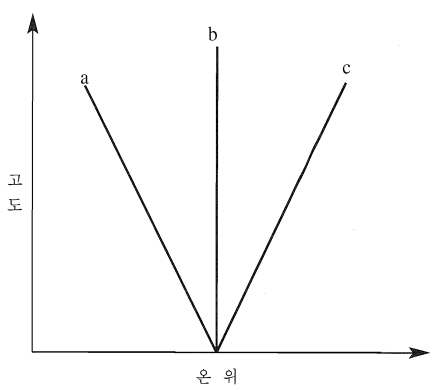
\includegraphics[width=0.8\textwidth]{./images/PT.png} 
				\end{figure}
				$ a: \frac{d\theta}{dz} > 0$ 안정, $ b: \frac{d\theta}{dz} = 0$ 중립, $ c: \frac{d\theta}{dz} < 0$ 불안정
			}
		\end{minipage}
	\end{tabular}
\end{frame}

